\subsection{Activity: String Telephone}
Materials required:
\begin{enumerate}
\item Two paper cups
\item A long piece of string
\end{enumerate}
Make a small hole at the bottom of each cup. Tie the ends of the string to the cups through these holes. Give one cup to your benchmate. Stand away from your benchmate to keep the string tight. Speak into one cup while your benchmate listens through the other cup. See Figure~\ref{stringtelephone}. Repeat the activity keeping the string loose. Compare the two sounds. 
\begin{figure}[h]
  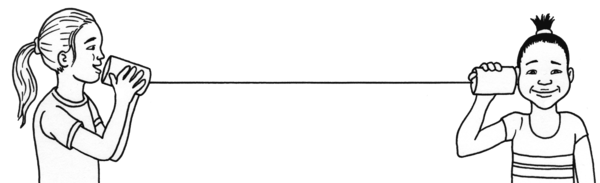
\includegraphics{stringtelephone}
  \caption{Image source: SASOL Inzalo Foundation}
  \label{fig:stringtelephone}
\end{figure}
\newthought{Observe:} Can your benchmate hear your voice when the string is tight? What happens to the sound when you loosen the string?

\newthought{Discuss:} When the string is tight, vibrations travel through the string from one cup to the other. When the string is loose, the vibrations do not travel as well. This activity shows that sound can travel through a solid medium.